\begin{figure*}
  \begin{center}
    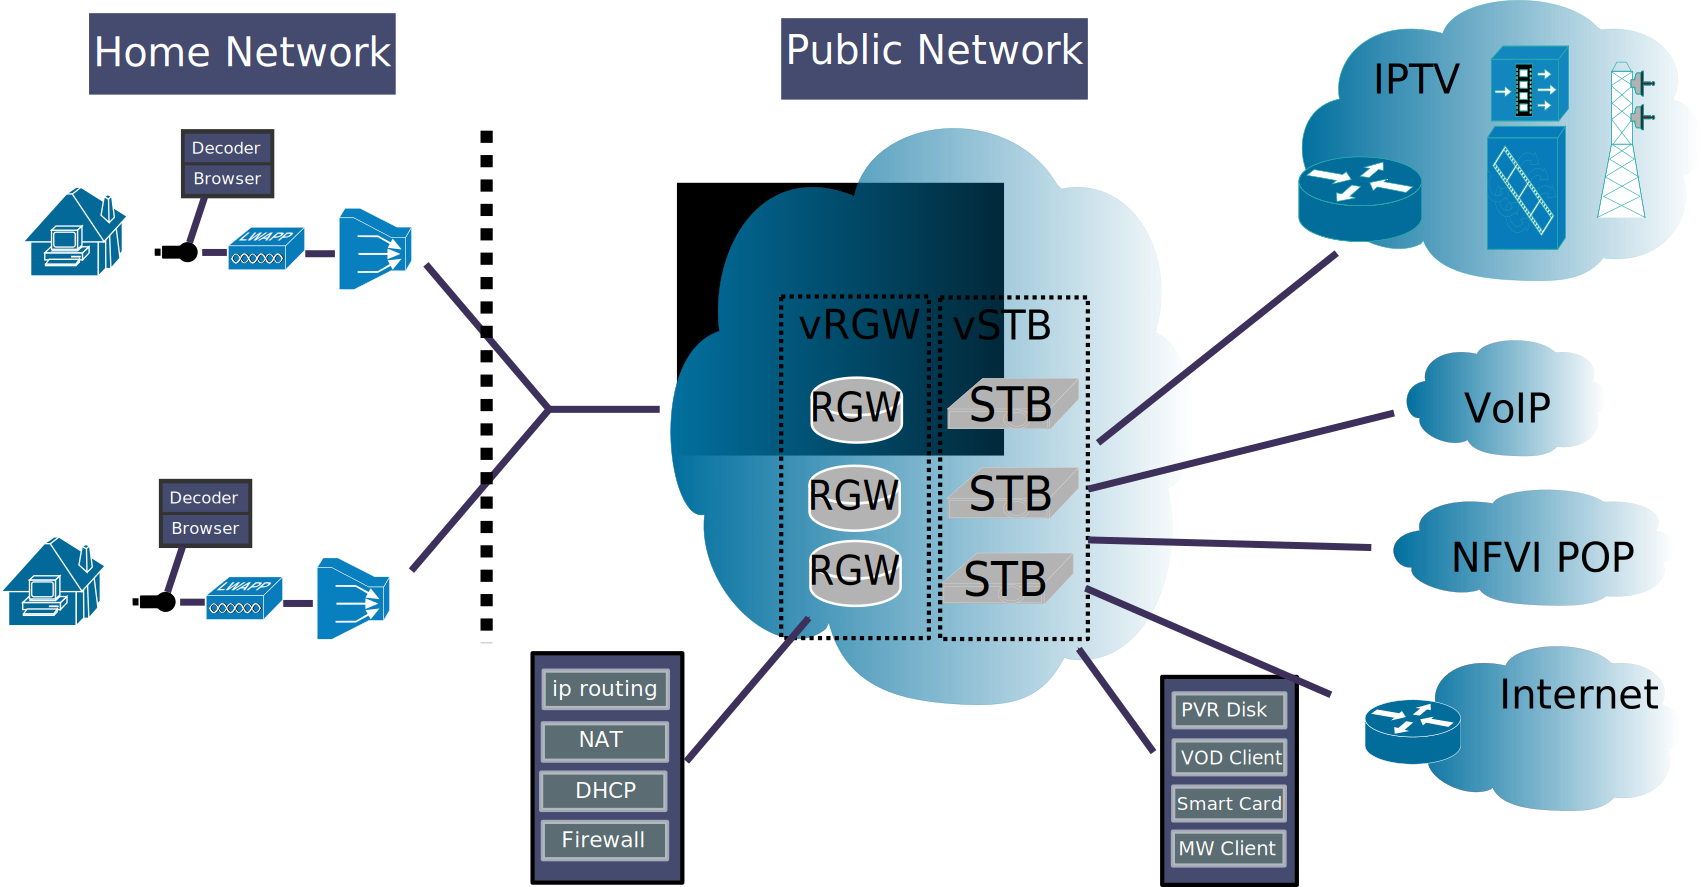
\includegraphics[width=0.75\textwidth]{fig/etsi-virtualization-home-env.pdf}
  \end{center}
  \caption{ Virtualization of the home environment according to ETSI.
    \label{fig:etsi-vision}
  }
\end{figure*}

Since the introduction of high speed Internet technologies such as xDSL and FTTx, End-Users' demands for Internet services grow at an exponential rate.
According to Akamai, the most popular Content Delivery Network (CDN) provider, the average bandwidth has continued to globally increase by 65\% in the second quarter of 2014 \cite{_akamais_2014} compared to 2013.

Once IP packets arrived at the customer's premises, they are processed by equipments such as Home Gateways (HG) and Set-Top Boxes (STB), to deliver content to a number of devices such as screens, smartphones, tablets, computers, mobile devices and security appliances.
HG and STB are placed on the last portion of the Service Provider's (SP) network under the conjoined responsibility of the End-User (EU) and the SP.
Functionally, the HG consists of the modem part that assures the translation of layers 1 and 2 between two heterogeneous networks: the SP's access network and the EU's home network.
The STB device is responsible for allowing access to IP video streamed services on their TV, such as live TV or Video On Demand (VOD).
Furthermore, HG \& STB usually consist of self-contained components, using internally stored firmware.
When new configuration updates are released, new model and firmware upgrades are being constantly pushed to the market.
The hardware and software fragmentation becomes more and more prominent, increasing operational expenses (OPEX). 

In the highly competitive industry of SP, where the arrival of a new player can be a game changer, new services and new norms are frequently rolled out.	
The impact on Customer Premise Equipment (CPE), like HG or STB, can be huge, as software updates can be insufficient to cover new requirements.
Updating hardware is vital, however this leads to high capital expenditure (CAPEX).
For instance, most STBs cannot decode the new video format standard  High Efficiency Video Coding (HEVC). 
The challenge for SP is threefold: they must find a way to tackle with disruptive changes brought by E.U. new expectations (like adopting 4K or 8K TV) and roll out new services to find new revenu streams while lowering expenses induced by replacing their network hardware.

The current trend of Cloud Computing that promotes the deployment of IT services on commodity servers has not reached the telco world so far, due to its lack of standardization and doubts regarding its ability to delivery carrier-grade services. Drawing on this observation, the European Telecommunications Standards Institute (ETSI) issued a seminal white paper \cite{_network_2012}, introducing the notion of Network Function Virtualization (NFV) and launched an Industry Specification Group for NFV, producing frequent publications.
The NFV concept aims at creating a reference architecture and a standardized approach to achieve carrier grade virtualization of existing hardware middle boxes on commodity servers.
Network equipment vitalization touches a broad range of devices, including HG and STB as ETSI mentions in the “Virtualization of the Home Environment” section of \cite{_network_2013}. 

As interest in NFV grows, several field studies are performed to verify it can be launched to market.
However, the transition from the current monolithic firmware based CPE to a proper full cloud solution is unlikely to happen immediately.

In this paper, we will study the feasibility of a NFV based HG. We propose a Virtual Network Function (VNF) integrated into a HG that will serve as a drop-in replacement for an existing function by leveraging the usage of Open Services Gateway initiative (OSGi\footnote{http://www.osgi.org/}) technology, for seamless HG exploitation within the cloud.
The rest of this paper is organized as follows.
Section II, will focus on the current and next generation Home Gateway architectures.
Section III will review existing approaches for visualizing CPEs in general.
Section IV will be dedicated to the description of our proof of concept, for which experimentations and results will be discussed in Section V.
Finally, Section VI will conclude and introduce future work.

